\documentclass[handout]{beamer}
\usepackage[orientation=portrait,size=A4]{beamerposter} 

\usepackage[utf8]{inputenc}
\usepackage[T1]{fontenc}
\usepackage{fontspec}
\usepackage[french]{babel}
\usepackage{graphicx}
\usepackage{array}
\usepackage{pifont}
\usepackage{amsmath, amssymb}
\usepackage{wrapfig}
\usepackage{mwe}
\usepackage{tikz}
\usetikzlibrary{calc}
\usepackage{pgfplots}
\pgfplotsset{compat=1.3}
\usepackage[compatibility=false,justification=centering]{caption}
\usepackage{mdframed}
\usepackage{amsmath}
\usepackage{amsfonts}
%\usepackage{pstricks,pst-plot,pstricks-add}

\newcommand{\tick}{\ding{52}}
\newcommand{\lnon}{\overline}
\newcommand{\ZZ}{{\mathbb{Z}/2\mathbb{Z}}}

\graphicspath{{./images/}}


\newcommand{\ensemble}[1]{{\left\lbrace{} #1 \right\rbrace{}}}
\newcommand{\ens}[1]{{\lbrace{} #1 \rbrace{}}}



\def\restriction#1#2{\mathchoice
              {\setbox1\hbox{${\displaystyle #1}_{\scriptstyle #2}$}
              \restrictionaux{#1}{#2}}
              {\setbox1\hbox{${\textstyle #1}_{\scriptstyle #2}$}
              \restrictionaux{#1}{#2}}
              {\setbox1\hbox{${\scriptstyle #1}_{\scriptscriptstyle #2}$}
              \restrictionaux{#1}{#2}}
              {\setbox1\hbox{${\scriptscriptstyle #1}_{\scriptscriptstyle #2}$}
              \restrictionaux{#1}{#2}}}
\def\restrictionaux#1#2{{#1\,\smash{\vrule height .8\ht1 depth .85\dp1}}_{\,#2}} 




%\usetheme{Boadilla}

\title{Optimisation de circuits logiques}
\author{Alexandre JANNIAUX}
\date{}

\begin{document}

\begin{frame}
  \maketitle
  \tableofcontents
\end{frame}

\section{Circuits logiques et fonctions combinatoires}
\begin{frame}
  \frametitle{Circuits logiques et fonctions combinatoires}
  
  \begin{itemize}

   \item Des intérêts industriels et scientifiques.
   \vfill\null
  
   \item \textbf{Circuit = Fonction logique}
   \begin{figure}[p]
   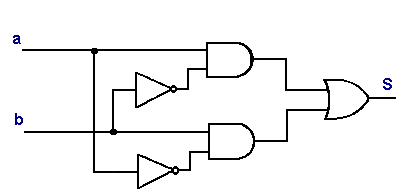
\includegraphics[width=8cm]{circuit_logique2.png}
   \caption{Exemple de circuit logique }
   \label{fig:circ1}
  \end{figure}
  
  \item Fonction canonique associée au circuit : \[f(a,b) = a\bar{b} + \bar{a}b\]
  \vfill\null

  \item\textbf{Problème de minimisation: } trouver la forme de la fonction avec le moins de terme possible.
  \vfill\null
  
  
  \item Les tests sont effectués sur un circuit de reconnaissance de nombre premier.

\end{itemize}
\end{frame}

\begin{frame}
  \frametitle{Représentation de la fonction}
  
  \textbf{Théorèmes :}
  \begin{mdframed}
  L'ensemble des fonctions booléennes $f(x_1, \cdots, x_n)$ est une $\ZZ$-algèbre de fonctions générée par les fonctions "littéraux" $X_i (x_1, \cdots, x_n) = x_1$.
  \end{mdframed} 
  
  \begin{mdframed}
  $\ensemble{\prod X_i^{\alpha_i} \mid \alpha_i\in \{-1,1\}}$, où $X_i^{-1} = \bar{X_i}$, est aussi cette algèbre. Donc 
  \[ f(x_1,\cdots, x_n) = \sum \prod_{i=1}^n X_i^{\alpha_i} \]
  \end{mdframed}
  
  
  %\begin{columns}
  %\begin{column}[t]{0.4\hsize}
  \begin{figure}[p]
  \begin{tikzpicture}[scale=1.5]
  (4,4)
      \coordinate (A) at (0,2,2);
      \coordinate (B) at (2,2,2);
      \coordinate (C) at (2,0,2);
      \coordinate (D) at (0,0,2);
      \coordinate (E) at (0,0,0);
      \coordinate (F) at (0,2,0);
      \coordinate (G) at (2,2,0);
      \coordinate (H) at (2,0,0);
      
      % ARETES DROITE
      \coordinate (AB) at ($ (A)!.5!(B) $);
      \coordinate (FG) at ($ (F)!.5!(G) $);
      \coordinate (BC) at ($ (B)!.5!(C) $);
      \coordinate (CD) at ($ (C)!.5!(D) $); 
      \coordinate (FG) at ($ (F)!.5!(G) $); 
      \coordinate (BG) at ($ (B)!.5!(G) $);
      \coordinate (DE) at ($ (D)!.5!(E) $);
      \coordinate (EF) at ($ (E)!.5!(F) $);      
      \coordinate (CH) at ($ (C)!.5!(H) $);
      
      \coordinate (ABFG) at ($ (AB)!.5!(FG) $);
      
	  \draw[very thick, ->] (0,0,0) -- (3,0,0) node [right] {$\vec{a}$};
  	  \draw[very thick, ->] (0,0,0) -- (0,3,0) node [left] {$\vec{b}$};
  	  \draw[very thick, ->] (0,0,0) -- (0,0,3) node [below right] {$\vec{c}$};      
      
      
      % ARMATURE CUBE GAUCHE
  	  \draw[thick](G)--(F)--(A)--(B)--(G)--(H)--(C)--(D)--(A);
  	  \draw[thick](B)--(C);
  	  \draw[gray](H)--(E)--(F);
 	  \draw[gray](E)--(D);
	  
	  % ELLIPSES GAUCHE
	  \draw[ultra thick] (D) circle(0.3) node [above left] {$\bar{a}\bar{b}c\quad$ };
	  %\draw[ultra thick] (BC) ellipse (0.3 and 1.3); % Verticales
  	  %\draw[ultra thick] (EF) ellipse (0.3 and 1.3); 
	  %\draw[ultra thick] (CD) ellipse (1.3 and 0.3); % Horizontales
	  %\draw[ultra thick] (FG) ellipse (1.3 and 0.3); 
	  \draw[ultra thick, rotate around={45:(CH)}] (CH)  ellipse (1 and 0.3) node[below right] {$a\bar{b}$}; % Oblique 
      %\draw[ultra thick, rotate around={45:(DE)}] (DE)  ellipse (1 and 0.3); % Oblique 		  	 
      \draw[ultra thick, rotate around={35:(ABFG)}] (ABFG)  ellipse (1.7 and 1.1) node {$a$}; 
	  	  
	  % ELLIPSES DROIT
	   	  
 	  
 	  % POINTS CUBE GAUCHE
  	  \filldraw(A) circle (0.15);
  	  \filldraw(B) circle (0.15);
  	  \filldraw(C) circle (0.15);
  	  \filldraw(D) circle (0.15);
  	  \filldraw(E) circle (0.15);
  	  \filldraw(F) circle (0.15);
  	  \filldraw(G) circle (0.15);
  	  \filldraw(H) circle (0.15) node[below right] {$H$};
  	  
  \end{tikzpicture}
  \end{figure}
  %\end{column}
  
  %\begin{column}[b]{0.6\hsize}
  \[ a\bar{b} = X_1 X_2 X_3 + X_1 X_2 \bar{X_3} \]
  %\end{column}
  %\end{columns}
  \vfill\null
  

\end{frame}

\section{M\'ethode de Quine-McCluskey}
\begin{frame}
  \frametitle{M\'ethode de Quine-McCluskey}
  
  \textbf{Expansion des cubes :}
  
     \begin{tikzpicture}[scale=2]
     (9,3)
      \coordinate (A) at (0,2,2);
      \coordinate (B) at (2,2,2);
      \coordinate (C) at (2,0,2);
      \coordinate (D) at (0,0,2);
      \coordinate (E) at (0,0,0);
      \coordinate (F) at (0,2,0);
      \coordinate (G) at (2,2,0);
      \coordinate (H) at (2,0,0);
      
      \coordinate (A2) at (6,2,2);
      \coordinate (B2) at (8,2,2);
      \coordinate (C2) at (8,0,2);
      \coordinate (D2) at (6,0,2);
      \coordinate (E2) at (6,0,0);
      \coordinate (F2) at (6,2,0);
      \coordinate (G2) at (8,2,0);
      \coordinate (H2) at (8,0,0);
      
      % ARETES DROITE
      \coordinate (BC2) at ($ (B2)!.5!(C2) $);
      \coordinate (CD2) at ($ (C2)!.5!(D2) $); 
      \coordinate (FG2) at ($ (F2)!.5!(G2) $); 
      \coordinate (BG2) at ($ (B2)!.5!(G2) $);
      \coordinate (DE2) at ($ (D2)!.5!(E2) $);
      \coordinate (EF2) at ($ (E2)!.5!(F2) $);      
      
      % ARMATURE CUBE GAUCHE
  	  \draw[thick](G)--(F)--(A)--(B)--(G)--(H)--(C)--(D)--(A);
  	  \draw[thick](B)--(C);
  	  \draw[gray](H)--(E)--(F);
 	  \draw[gray](E)--(D);
 	  
 	  % ARMATURE CUBE DROIT
 	  \draw[thick](G2)--(F2)--(A2)--(B2)--(G2)--(H2)--(C2)--(D2)--(A2);
  	  \draw[thick](B2)--(C2);
  	  \draw[gray](H2)--(E2)--(F2);
 	  \draw[gray](E2)--(D2);
 	  
	  % FLECHE
	  \draw[ultra thick](4,1.4,2)--(5,1.4,2)--(5,1.6,2)--(5.5,1.2,2)--(5,0.8,2)--(5,1,2)--(4,1,2);
	  
	  % ELLIPSES GAUCHE
	  \draw[ultra thick] (BC2) ellipse (0.3 and 1.3); % Verticales
  	  \draw[ultra thick] (EF2) ellipse (0.3 and 1.3); 
	  \draw[ultra thick] (CD2) ellipse (1.3 and 0.3); % Horizontales
	  \draw[ultra thick] (FG2) ellipse (1.3 and 0.3); 
	  \draw[ultra thick, rotate around={45:(BG2)}] (BG2)  ellipse (1 and 0.3); % Oblique 
      \draw[ultra thick, rotate around={45:(DE2)}] (DE2)  ellipse (1 and 0.3); % Oblique 		  	  
	  	  
	  % ELLIPSES DROIT
	   	  
 	  
 	  % POINTS CUBE GAUCHE
  	  \draw(A) circle (0.15) node[below left] {$A$};
  	  \filldraw(B) circle (0.15) node[below right] {$B$};
  	  \filldraw(C) circle (0.15) node[below right] {$C$};
  	  \filldraw(D) circle (0.15) node[below left] {$D$};
  	  \filldraw(E) circle (0.15) node[below right] {$E$};
  	  \filldraw(F) circle (0.15) node[above left] {$F$};
  	  \filldraw(G) circle (0.15) node[above right] {$G$};
  	  \draw(H) circle (0.15) node[below right] {$H$};
  	  
  	  % POINTS CUBE DROIT
  	  \draw(A2) circle (0.15);
  	  \filldraw(B2) circle (0.15);
  	  \filldraw(C2) circle (0.15);
  	  \filldraw(D2) circle (0.15);
  	  \filldraw(E2) circle (0.15);
  	  \filldraw(F2) circle (0.15);
  	  \filldraw(G2) circle (0.15);
  	  \draw(H2) circle (0.15);
     \end{tikzpicture}
     \vfill\null

  \textbf{Performances :}     
     
     \begin{columns}
     	\begin{column}[t]{0.5\hsize}
	     \begin{tikzpicture}[scale=0.8]
    	 \begin{axis}[
	ymode=log,
	extra tick style={grid=major},
	title=Circuit premier,
	xlabel={nombre de variables},
	ylabel={temps ($s$)}]

\addplot table {images/expand_bench.dat};
	
\end{axis}
	
%\draw plot coordinates {
%(0,0) 
%(1,0) 
%(2,0) 
%(3,0)
%(4,0.003) 
%(5,0.014) 
%(6,0.07) 
%(7,0.33) 
%(8,1.8) 
%(9,10.8) %};
%(10,56.6)};
	     \end{tikzpicture}
	     \end{column}

     
	     \begin{column}[t]{0.5\hsize}
	     \begin{tikzpicture}[scale=0.8]
    	 \begin{axis}[
	xmode=log,
	ymode=log,
	extra tick style={grid=major},
	title=Circuit premier,
	xlabel={nombre de cubes},
	ylabel={temps ($s$)}]

\addplot table {images/expand_bench_cube.dat};
	
\end{axis}
	
%\draw plot coordinates {
%(0,0) 
%(1,0) 
%(2,0) 
%(3,0)
%(4,0.003) 
%(5,0.014) 
%(6,0.07) 
%(7,0.33) 
%(8,1.8) 
%(9,10.8) %};
%(10,56.6)};
	     \end{tikzpicture}
    	 \end{column} 
	  \end{columns}
	  
	\vfill\null
	\textbf{Conclusion : } Croissance exponentielle en le nombre de variables.
	  
%  \large{\textbf{Exemple :}} \[ f(x_1,\cdots,x_6) = \sum m(36, 44, 51, 60) \]
%
%  
%  \begin{minipage}[b]{0.5\hsize}\centering
%    \begin{tabular}{rl}
%      36: & 100100  \tick \\ \hline 
%      44: & 101100  \tick \\ 
%      51: & 110011   \\ \hline
%      60: & 111100 \tick
%    \end{tabular}
%  \end{minipage}
%  %
%  \begin{minipage}{0.4\hsize}\centering
%    \begin{tabular}{rl}
%      36,44: & 10\_100  \\ \hline 
%      44,60: & 1\_1100    
%    \end{tabular}
%  \end{minipage}
  
  %\large{\textbf{Idée :}} Une fonction combinatoire est définie par le langage accepté (couverture).
  
  %=> On utilise l'algèbre de Boole pour simplifier les expressions
  
  %\large{\textbf{Algorithme :}}
  %\begin{enumerate}
  %   \item 
  %\end{enumerate}
\end{frame}

\begin{frame}
  \frametitle{Méthode de Quine-McCluskey}
  \textbf{Suppression des redondances inutiles : }
   \vfill\null  
  \begin{tikzpicture}[scale=2]
  (9,3)
      \coordinate (A) at (0,2,2);
      \coordinate (B) at (2,2,2);
      \coordinate (C) at (2,0,2);
      \coordinate (D) at (0,0,2);
      \coordinate (E) at (0,0,0);
      \coordinate (F) at (0,2,0);
      \coordinate (G) at (2,2,0);
      \coordinate (H) at (2,0,0);
      
      \coordinate (A2) at (6,2,2);
      \coordinate (B2) at (8,2,2);
      \coordinate (C2) at (8,0,2);
      \coordinate (D2) at (6,0,2);
      \coordinate (E2) at (6,0,0);
      \coordinate (F2) at (6,2,0);
      \coordinate (G2) at (8,2,0);
      \coordinate (H2) at (8,0,0);
      
      % ARETES GAUCHE
      \coordinate (BC) at ($ (B)!.5!(C) $);
      \coordinate (CD) at ($ (C)!.5!(D) $); 
      \coordinate (FG) at ($ (F)!.5!(G) $); 
      \coordinate (BG) at ($ (B)!.5!(G) $);
      \coordinate (DE) at ($ (D)!.5!(E) $);
      \coordinate (EF) at ($ (E)!.5!(F) $);      
      
      % ARETES DROITE
      \coordinate (BC2) at ($ (B2)!.5!(C2) $);
      \coordinate (CD2) at ($ (C2)!.5!(D2) $); 
      \coordinate (FG2) at ($ (F2)!.5!(G2) $); 
      \coordinate (BG2) at ($ (B2)!.5!(G2) $);
      \coordinate (DE2) at ($ (D2)!.5!(E2) $);
      \coordinate (EF2) at ($ (E2)!.5!(F2) $);      
      
      
      % ARMATURE CUBE GAUCHE
  	  \draw[thick](G)--(F)--(A)--(B)--(G)--(H)--(C)--(D)--(A);
  	  \draw[thick](B)--(C);
  	  \draw[gray](H)--(E)--(F);
 	  \draw[gray](E)--(D);
 	  
 	  % ARMATURE CUBE DROIT
 	  \draw[thick](G2)--(F2)--(A2)--(B2)--(G2)--(H2)--(C2)--(D2)--(A2);
  	  \draw[thick](B2)--(C2);
  	  \draw[gray](H2)--(E2)--(F2);
 	  \draw[gray](E2)--(D2);
 	  
	  % FLECHE
	  \draw[ultra thick](4,1.4,2)--(5,1.4,2)--(5,1.6,2)--(5.5,1.2,2)--(5,0.8,2)--(5,1,2)--(4,1,2);
	  
	
	  % ELLIPSES GAUCHE
	  \draw[ultra thick] (BC) ellipse (0.3 and 1.3); % Verticales
  	  \draw[ultra thick] (EF) ellipse (0.3 and 1.3); 
	  \draw[ultra thick] (CD) ellipse (1.3 and 0.3); % Horizontales
	  \draw[ultra thick] (FG) ellipse (1.3 and 0.3); 
	  \draw[ultra thick, rotate around={45:(BG)}] (BG)  ellipse (1 and 0.3); % Oblique 
      \draw[ultra thick, rotate around={45:(DE)}] (DE)  ellipse (1 and 0.3); % Oblique 		  
	  
	  
	  % ELLIPSES DROITE
	  %\draw[ultra thick] (BC2) ellipse (0.3 and 1.3); % Verticales
  	  \draw[ultra thick] (EF2) ellipse (0.3 and 1.3); 
	  \draw[ultra thick] (CD2) ellipse (1.3 and 0.3); % Horizontales
	  %\draw[ultra thick] (FG2) ellipse (1.3 and 0.3); 
	  \draw[ultra thick, rotate around={45:(BG2)}] (BG2)  ellipse (1 and 0.3); % Oblique 
      %\draw[ultra thick, rotate around={45:(DE2)}] (DE2)  ellipse (1 and 0.3); % Oblique 		  	  
	  	  
	  % ELLIPSES DROIT
	   	  
 	  
 	  % POINTS CUBE GAUCHE
  	  \draw(A) circle (0.15);
  	  \filldraw(B) circle (0.15);
  	  \filldraw(C) circle (0.15);
  	  \filldraw(D) circle (0.15);
  	  \filldraw(E) circle (0.15);
  	  \filldraw(F) circle (0.15);
  	  \filldraw(G) circle (0.15);
  	  \draw(H) circle (0.15);
  	  
  	  % POINTS CUBE DROIT
  	  \draw(A2) circle (0.15);
  	  \filldraw(B2) circle (0.15);
  	  \filldraw(C2) circle (0.15);
  	  \filldraw(D2) circle (0.15);
  	  \filldraw(E2) circle (0.15);
  	  \filldraw(F2) circle (0.15);
  	  \filldraw(G2) circle (0.15);
  	  \draw(H2) circle (0.15);
  \end{tikzpicture}  
  \vfill\null  
  
  \par
  \textbf{Méthodes :}
  \begin{itemize}
  	\item Développement naïf : débordement pour $n\geq 5$
  	\item Backtracking : $t>20600s$ pour $n\geq 7$
  	\item Algorithme de couverture minimale glouton
  \end{itemize} 
  \vfill\null 
  
  \textbf{Performances}
  \par
  \begin{columns}
  	  \begin{column}[t]{0.5\hsize}
	  \begin{tikzpicture}[scale=0.8]
	  \begin{axis}[
	ymode=log,
	extra tick style={grid=major},
	title=Heuristique irredondance,
	xlabel={nombre de variables},
	ylabel={temps ($s$)}]

\addplot table {images/irredundant_bench_heuristic.dat};
	
\end{axis}
	  \end{tikzpicture}
	  \end{column}
	  
	  \begin{column}[t]{0.5\hsize}
	  \begin{tikzpicture}[scale=0.8]
	  \begin{axis}[
	xmode=log,
    ymode=log,
	extra tick style={grid=major},
	title=Heuristique irredondance,
	xlabel={nombre de cubes},
	ylabel={temps ($s$)}]

\addplot table {images/irredundant_bench_heuristic_cube.dat};
	
\end{axis}
	  \end{tikzpicture}
	  \end{column}
	\end{columns}
	  
%  
%  \begin{minipage}[c][6cm]{\hsize}\centering
%    \begin{tabular}{|l|c|c|c|c|}
%      \hline %
%      Implicants & 36 & 44 & 51 & 60  \\ \hline
%      51 &  &  & X &  \\ \hline
%      36,44 & X & X &  &    \\ \hline
%      44,60 &  & X &  & X \\ \hline
%    \end{tabular}
%    \newline
%    
%  \end{minipage}
%
%  \textbf{Méthode de Petrick :} exacte, exemple
%  \[ g \equiv (P_1+P_2)(P_1+P_4+P_4)\cdots(P_7+P_9) \]
%
%  \textbf{Approximation :}
%  \begin{itemize}
%  \item plus rapide
%  \item approximation en $H_n$
%  \item adapté à plusieurs itérations
%  \end{itemize}
\end{frame}

\begin{frame}
  \frametitle{Résultats}
	\begin{columns}
	  \begin{column}[t]{0.5\hsize}
	  \begin{tikzpicture}[scale=0.8]
		  \begin{axis}[
	xmode=log,
	ymode=log,
	extra tick style={grid=major},
	title=Minimisation,
	xlabel={nombre de cubes initial},
	ylabel={nombre de cubes final}]

\addplot table {images/bench_cube_mini.dat};
	
\end{axis}
	  \end{tikzpicture}  
	  \end{column}
	  
	  \begin{column}[t]{0.5\hsize}
	  \begin{tikzpicture}[scale=0.8]
		  \begin{axis}[
	ymode=log,
  grid=major,
	extra tick style={grid=major},
	title=Minimisation,
	xlabel={nombe de variables},
	ylabel={nombre de cubes}]

\addplot table {images/bench_cube_mini_n_start.dat};
\addplot table {images/bench_cube_mini_n_end.dat};
	
\end{axis}

	  \end{tikzpicture}  
	  \end{column}
	 \end{columns}
	 
	 \vfill\null
	 \par
	\begin{columns}
	  \begin{column}[t]{0.5\hsize}
	  \begin{tikzpicture}[scale=0.8]
		  \begin{axis}[
  xmode=log,
  ymode=log,
  grid=major,
	extra tick style={grid=major},
	title=Efficacité,
	xlabel={nombre de littéraux initial},
	ylabel={nombre de littéraux final}]

\addplot table {images/bench_literal_mini_n.dat};
	
\end{axis}

	  \end{tikzpicture}  
	  \end{column}
	  
	  \begin{column}[t]{0.5\hsize}
	  \begin{tikzpicture}[scale=0.8]
		  \begin{axis}[
	ymode=log,
  grid=major,
	extra tick style={grid=major},
	title=Évolution de l'efficacité,
	xlabel={nombre de variables},
	ylabel={nombre de littéraux}]

\addplot table {images/bench_literal_mini_start.dat};
\addplot table {images/bench_literal_mini_end.dat};
	
\end{axis}

	  \end{tikzpicture}  
	\end{column}
\end{columns}

\begin{tikzpicture}[scale=0.8]
	\begin{axis}[
	xmode=log,
	ymode=log,
  grid=major,
	extra tick style={grid=major},
	title=Minimisation,
	xlabel={nombre de cubes initial},
	ylabel={nombre de cubes final}]

\addplot table {images/bench_mini_logdiff.dat};
	
\end{axis}

\end{tikzpicture}  

\end{frame}

\section{Généralisation à tout circuit}
\begin{frame}
  \frametitle{Fonctions multivaluées}

  \textbf{Définition :}
  \begin{mdframed}
  \[ f: \mathcal{P}_1 \times \cdots \times \mathcal{P}_n \longrightarrow \mathbb{B}^m \]
  \end{mdframed}

  \textbf{Littéraux :} 
  \begin{mdframed}
  \[{X_i^{S_i} = %
  \begin{cases}
    1 \text{ si } X_i \in S_i \\
    0 \text{ sinon}
  \end{cases}
  \quad \text{où } X_i \in \mathcal{P}_i \text{ et } \mathcal{S}_i \subset \mathcal{P}_i} \]
    \end{mdframed}  
  
  
  \begin{figure}
  \centering
	  \begin{tikzpicture}[scale=2]  
  		(4,3)
      \coordinate (A) at (0,2,2);
      \coordinate (B) at (2,2,2);
      \coordinate (C) at (2,0,2);
      \coordinate (D) at (0,0,2);
      \coordinate (E) at (0,0,0);
      \coordinate (F) at (0,2,0);
      \coordinate (G) at (2,2,0);
      \coordinate (H) at (2,0,0);
      
      \coordinate (I) at (4,2,2);
      \coordinate (J) at (4,2,0);
      \coordinate (K) at (4,0,0);
      \coordinate (L) at (4,0,2);
      
        
      
      % ARMATURE CUBE GAUCHE
  	  \draw[thick](G)--(F)--(A)--(B)--(G)--(H);
  	  \draw[thick](C)--(D)--(A);
  	  \draw[gray](H)--(C);
  	  \draw[thick](B)--(C);
  	  \draw[gray](K)--(H)--(E)--(F);
 	  \draw[gray](E)--(D);
 	  
 	  \draw[thick](I)--(J)--(K)--(L)--(I);
 	  \draw[thick](B)--(I);
 	  \draw[thick](C)--(L);
 	  \draw[thick](J)--(G);
	 
 	  
	  % POINTS CUBE DROIT
  	  \draw(A) circle (0.15);
  	  \draw(B) circle (0.15);
  	  \draw(C) circle (0.15);
  	  \filldraw(D) circle (0.15);
  	  \filldraw(E) circle (0.15);
  	  \draw(F) circle (0.15);
  	  \filldraw(G) circle (0.15);
  	  \draw(H) circle (0.15);
  	  \draw(I) circle (0.15);
  	  \draw(J) circle (0.15);
  	  \filldraw(K) circle (0.15);
  	  \filldraw(L) circle (0.15);
  	  
  	  \draw[very thick, ->] (0,0,0) -- (6,0,0) node [right] {$X_1$};
  	  \draw[very thick, ->] (0,0,0) -- (0,3,0) node [left] {$X_2$};
  	  \draw[very thick, ->] (0,0,0) -- (0,0,3) node [left] {$X_3$};
	  \end{tikzpicture}
	  \caption{Représentation de $f = X_1^\ens{0,2} X_2^\ens{0} + X_1^\ens{1} X_2^\ens{1}X_3^\ens{0}$}
	\end{figure}

  \textbf{Décomposition de Shannon :}
  \begin{mdframed}
  \[ \bigcup_{i=1}^n c_i = 1 \implies f \equiv \bigcup_{i=1}^{n} c_i \cap \restriction{f}{c_i} \]
  \end{mdframed}

\end{frame}

\begin{frame}
  \frametitle{Espresso}

  \[ \bigcup_{i=1}^n c_i = 1 \implies f \equiv \bigcup_{i=1}^{n} c_i \cap \restriction{f}{c_i}\]

  \textbf{Atout :} Paradigme diviser pour régner
  \par Chaque étape est divisée en plus petites.
	
  \textbf{Opérations :}  
  \begin{itemize}
  \item Expansion améliorée.
  \item Élimination des redondances.
  \item Réduction des cubes.
  \end{itemize}
  
  
  
\end{frame}

\begin{frame}
  \frametitle{Conclusion}

  \begin{itemize}
  \item Problème difficile à résoudre de façon naïve.
  \item Intéressant : tourne autour de plusieurs grands problèmes.
  \item Très bien maitrisé aujourd'hui.
  \item D'autres applications : Arbre de décision multivalué, etc.
  \end{itemize}

\end{frame}

\end{document}
